\documentclass[10pt]{article}
\usepackage[margin=0.8in]{geometry}
\usepackage{graphicx,longtable,hyperref}
\hypersetup{colorlinks=true,urlcolor=blue,linkcolor=black,pdfauthor={Libor Burny Burian}}
\setlength{\parindent}{0pt}\setlength{\parskip}{5pt}\setlength{\emergencystretch}{3em}
\title{Can a 32-component algebra help a neural network compare spatially selected objects?}
\author{Libor \textquotedblleft Burny\textquotedblright\ Burian}
\date{26 November 2026}
\begin{document}\maketitle
\begin{abstract}
A noisy sensor observes one component of an unknown linear mixing of an object's excitation. A graph neural network must identify two objects through intermediary landmarks and predict whether they have the same hidden type. We cross the multiplication rule used by the sensor with the rule used to tie neural weights. This synthetic intervention measures whether compatible weight sharing improves end-to-end decisions. The pilot classified 89.16\% of 2,048 unseen scenes correctly and answered both mates correctly in 82.23\% of families. The constant control scored 50.00\% and the privileged sensor-and-geometry oracle scored 93.55\%. On unseen sensor coordinates accuracy was 89.79\%. Seed 42 is excluded from all confirmatory contrasts. The registered crossover awaits complete paired worlds.
\end{abstract}
\section{Motivation and related work}
Spatial structure can restrict which interactions a model must learn. Relational scene benchmarks [10], message passing [11] and distance-conditioned equivariant networks [12] motivate our scene generator and graph processor. We study a second, independent assumption about which observable channels share parameters. Real convolutional and residual networks [3,4], complex [5], quaternion [6], octonion [7] and sedenion networks [8,9] establish precedents for the smaller component counts. Our contribution is the combination of a 32-component trainable graph classifier, paired counterfactual scenes and a crossover intervention. We make no priority claim for 32-component neural layers.
\section{Method}
Starting with real scalars, double five times using
\[
 (a,b)(c,d)=(ac-\bar d b,\;da+b\bar c).
\]
For basis elements $e_i e_j=s_{ij}e_{i\oplus j}$, a learned left multiplier maps $x$ to $y_k=\sum_j s_{k\oplus j,j}w_{k\oplus j}x_j$ [1,2]. One block of 32 real trainable scalars supplies all entries of a $32\times32$ matrix. Ordinary tensor contraction computes that matrix on the accelerator. Each layer has explicit operand order. This construction needs neither associativity nor a multiplicative inverse. Five doublings do not imply five-dimensional spatial equivariance.
 
Each world draws a unit filter $w$ with zero scalar component and equal squared energy in the lower and upper halves. For object type $b\in\{-1,+1\}$, Gaussian excitation $x$ and index $k$, the observed scalar is $z=b(w\star x)_k+\epsilon$, with $\epsilon\sim N(0,0.1^2)$. The canonical sensor uses an independent scalar implementation [15]. The random sensor flips all six signs of 60 uniformly sampled upper basis triples while preserving the ordered-product support, the identity, the imaginary squares, and the lower 16-component table. The randomized rule is a signed bilinear control.

Draw two beacons, four landmarks and eight objects uniformly in the plane. Reject layouts with coinciding nearest choices or a nearest/second-nearest distance margin of at most 0.035 at a selected hop. Half the objects have each type. From each beacon follow its nearest landmark and then its nearest object. Equality of the two object types is the binary target. Swapping the entire reading of a selected object with an opposite-type distractor flips the answer. Full families stay within the same split. An order-independent readings-only predictor or geometry-only predictor makes exactly one correct decision per family.

The encoder mixes the excitation with four learned channel projections, reads each at the observed coordinate and supplies the projections, their products with $z$, and $z$ to a nonlinear MLP. A landmark pools object features and a beacon pools landmark features using a learned function of squared distance plus a learned negative distance slope. Signed linear residual updates transform the pooled features. A real MLP reads the sum and elementwise product of both beacon embeddings. Using distances and symmetric aggregates makes the full prediction invariant to a common planar isometry and within-role index permutations.
\begin{center}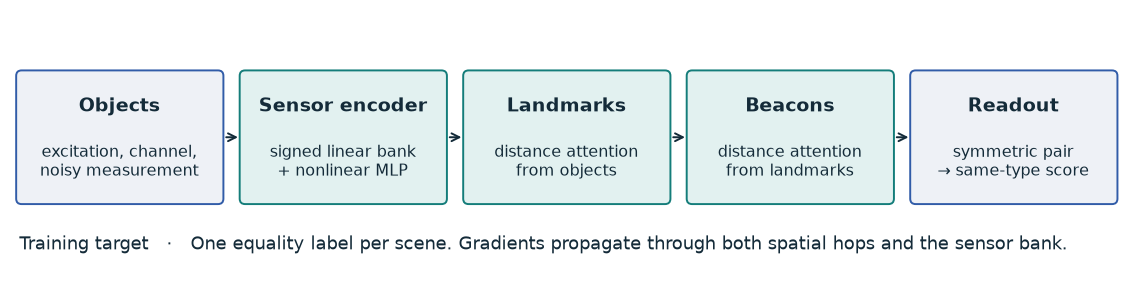
\includegraphics[width=.94\linewidth,height=.29\textheight,keepaspectratio]{docs/figures/architecture.png}
\\{\small Figure 1. End-to-end classifier. Object types and selection indices are withheld from the learner.}\end{center}

\section{Experiment and falsification criteria}
Each primary world has 1,024 training, 256 validation and 1,024 test families. Withhold sensor coordinates 12--15 and 28--31 during training. Evaluate fresh scenes with these coordinates and scenes with 16 objects separately. Both matched and mismatched networks receive identical underlying geometry, labels, excitations, noise and optimizer settings. Fit 80 epochs of AdamW, initial learning rate 0.003, weight decay 0.0001, batch size 128 scenes and cosine decay. Break ties in maximum validation accuracy in favor of the earliest epoch. A frozen random encoder with trained readout, one-hop network, shallow coordinate-aware set network, unrestricted real, low-rank real and sedenion learners control different aspects of the architecture.

Seed 42 is a development pilot. Compute two-sided 95\% Student intervals over paired differences from eight independent confirmatory worlds. A matched learner must have a lower bound above 60\% for task success. Both directional crossover lower bounds must exceed one percentage point for a matching claim. Both depth comparisons must have positive lower bounds for the multistage attribution. Incomplete seed sets defer decisions [16]. Data-size sensitivity and the individual controls are descriptive. Multiple testing, resource limits and optimization sensitivity constrain interpretation.

Auxiliary multiplier and unrestricted bilinear least-squares fits test algebraic recovery. Separate transfer experiments compare structured residual image classifiers on CIFAR-10 and its duplicate-corrected ciFAIR-10 test set [4,14]. Superpixel classification uses the published split [13] with a learned color input and a graph-mean readout. The simulator supplies no sensor rule for natural images. The registered transfer contrast evaluates canonical versus randomized sharing on ciFAIR-10.
\section{Results and claims}
The pilot classified 89.16\% of 2,048 unseen scenes correctly and answered both mates correctly in 82.23\% of families. The constant control scored 50.00\% and the privileged sensor-and-geometry oracle scored 93.55\%. On unseen sensor coordinates accuracy was 89.79\%. Seed 42 is excluded from all confirmatory contrasts. The registered crossover awaits complete paired worlds.
\begin{longtable}{p{.43\linewidth}rrrr}
\hline Task / model / rule & Worlds & Params & Test & 95\% interval\\\hline\endhead
scene / cd32 / cd32 / 1024 families (pilot) & 1 & 3801 & 89.16\% & ---\\
\hline\end{longtable}
\begin{longtable}{p{.37\linewidth}rp{.11\linewidth}p{.17\linewidth}l}
\hline Endpoint & N & Estimate & 95\% interval & Decision\\\hline\endhead
Matched canonical accuracy & 0 & pending & --- & pending\\
Matched randomized accuracy & 0 & pending & --- & pending\\
Canonical minus randomized on canonical sensors & 0 & pending & --- & pending\\
Randomized minus canonical on randomized sensors & 0 & pending & --- & pending\\
Canonical minus frozen & 0 & pending & --- & pending\\
Canonical minus validation-selected shallow control & 0 & pending & --- & pending\\
Canonical minus randomized on ciFAIR-10 & 0 & pending & --- & pending\\
\hline\end{longtable}
\begin{center}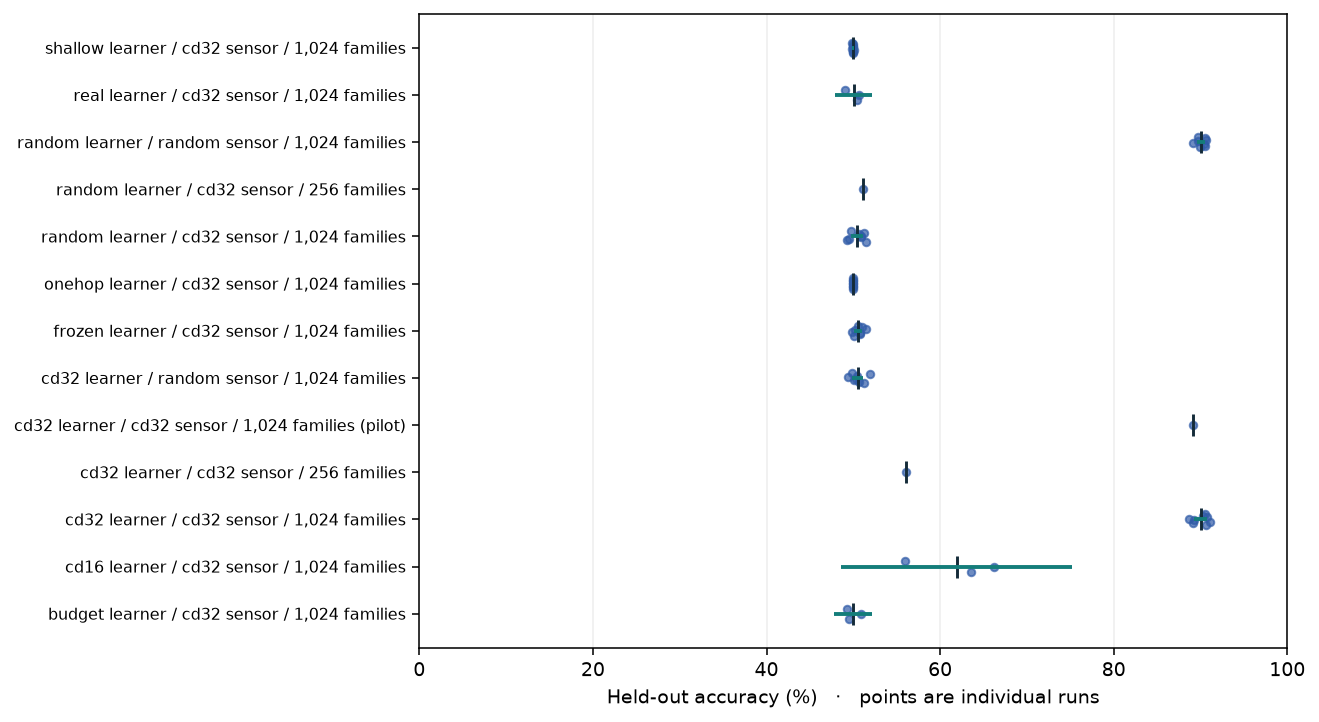
\includegraphics[width=.94\linewidth,height=.29\textheight,keepaspectratio]{docs/figures/scores.png}
\\{\small Each dot is a held-out world. The vertical tick denotes its group's arithmetic mean.}\end{center}
\begin{center}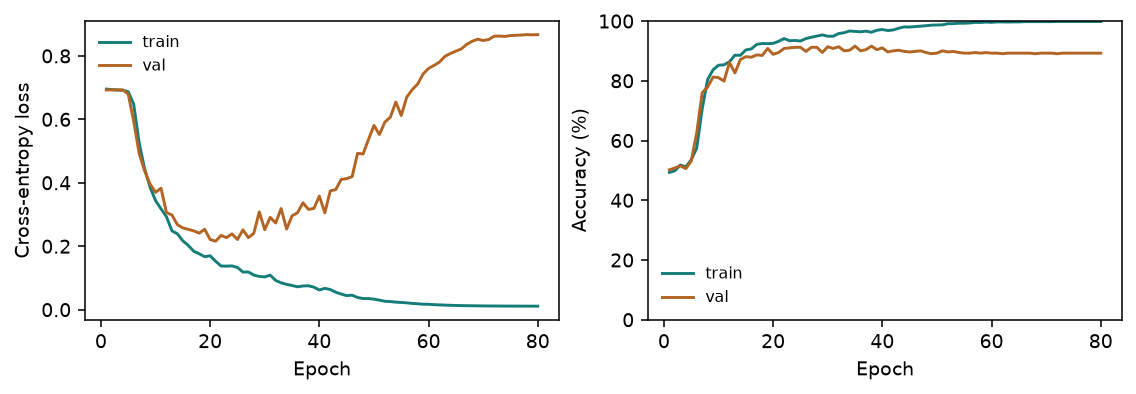
\includegraphics[width=.94\linewidth,height=.29\textheight,keepaspectratio]{docs/figures/learning.png}
\\{\small Pilot binary cross entropy and accuracy by epoch, from the timestamped training log.}\end{center}
\begin{center}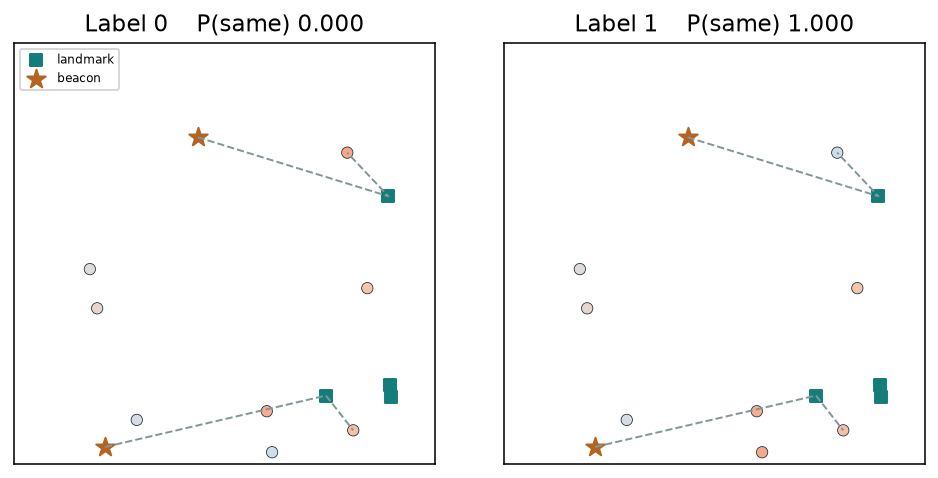
\includegraphics[width=.94\linewidth,height=.29\textheight,keepaspectratio]{docs/figures/example.png}
\\{\small A fixed held-out family. Circles show object readings, square markers landmarks and stars beacons. Dashed paths show ground-truth selections.}\end{center}
\subsection*{Independent algebra diagnostic}
\begin{longtable}{lllrrrr}
\hline Task & Teacher & Learner & N & Worlds & NMSE & Basis\\\hline\endhead
multiplier & cd32 & cd32 & 2 & 3 & 3.57e-31 & ---\\
multiplier & cd32 & random & 2 & 3 & 1.77 & ---\\
multiplier & cd32 & real & 2 & 3 & 0.933 & ---\\
multiplier & cd32 & cd32 & 8 & 3 & 2.57e-31 & ---\\
multiplier & cd32 & random & 8 & 3 & 0.943 & ---\\
multiplier & cd32 & real & 8 & 3 & 0.733 & ---\\
multiplier & cd32 & cd32 & 32 & 3 & 2.61e-31 & ---\\
multiplier & cd32 & random & 32 & 3 & 0.847 & ---\\
multiplier & cd32 & real & 32 & 3 & 1.97e-28 & ---\\
multiplier & cd32 & cd32 & 128 & 3 & 3.73e-31 & ---\\
multiplier & cd32 & random & 128 & 3 & 0.825 & ---\\
multiplier & cd32 & real & 128 & 3 & 2.32e-31 & ---\\
multiplier & random & cd32 & 2 & 3 & 1.52 & ---\\
multiplier & random & random & 2 & 3 & 3.3e-31 & ---\\
multiplier & random & real & 2 & 3 & 0.937 & ---\\
multiplier & random & cd32 & 8 & 3 & 0.938 & ---\\
multiplier & random & random & 8 & 3 & 2.37e-31 & ---\\
multiplier & random & real & 8 & 3 & 0.74 & ---\\
multiplier & random & cd32 & 32 & 3 & 0.843 & ---\\
multiplier & random & random & 32 & 3 & 2.67e-31 & ---\\
multiplier & random & real & 32 & 3 & 1.71e-28 & ---\\
multiplier & random & cd32 & 128 & 3 & 0.822 & ---\\
multiplier & random & random & 128 & 3 & 3.11e-31 & ---\\
multiplier & random & real & 128 & 3 & 2.34e-31 & ---\\
product & cd32 & bilinear & 256 & 3 & 0.742 & 826.0\\
product & cd32 & shuffled & 256 & 3 & 1.38 & 17.3\\
product & cd32 & bilinear & 1024 & 3 & 4.69e-27 & 1024.0\\
product & cd32 & shuffled & 1024 & 3 & 3.84e+03 & 15.0\\
product & cd32 & bilinear & 2048 & 3 & 1.95e-30 & 1024.0\\
product & cd32 & shuffled & 2048 & 3 & 2.07 & 16.0\\
product & cd32 & analytic & 0 & 3 & 0 & 1024.0\\
\hline\end{longtable}

\section{Discussion, limitations and conclusion}
A successful crossover identifies an effect of matching the assumed interaction rule to this simulator under this training recipe. The treatment changes the tied matrices throughout the encoder and message blocks, so a net effect alone does not localize the mechanism. Scene families share a world-specific filter, and evaluation addresses fresh scenes within each trained world. The task supplies object segmentation, roles and coordinates. Natural images require separate transfer evidence. The factorization and sample count of the real controls affect representational capacity and optimization. The privileged oracle knows the measurement filter and nearest paths. Noise makes even its decisions fallible. Diagnostic product recovery and gradients alone cannot establish that a scene classifier learned the task.

\section*{Appendix: replication and evidence}
The public repository contains the full seed matrix, pinned environment, checkpoint configurations, training and validation logs, individual test predictions, both mates of fixed example families, and regeneration code as runs are published. To regenerate this paper and every table and figure, run \texttt{uv run trig32 report} at the repository root. See the \href{https://github.com/BurnyCoder/trigintaduonion-neural-network}{source and run guide} and \href{https://burnycoder.github.io/trigintaduonion-neural-network/}{interactive explorer}.
\section*{References}
\begin{enumerate}
\item \href{https://arxiv.org/abs/math/0511691}{Biss, Dugger and Isaksen. Large annihilators in Cayley--Dickson algebras. Definition 2.1.}
\item \href{https://arxiv.org/abs/1405.6888}{Saniga et al. Cayley--Dickson algebras and finite geometry.}
\item \href{https://leon.bottou.org/papers/lecun-98h}{LeCun et al. Gradient-based learning applied to document recognition.}
\item \href{https://arxiv.org/abs/1512.03385}{He et al. Deep residual learning for image recognition.}
\item \href{https://arxiv.org/abs/1705.09792}{Trabelsi et al. Deep complex networks.}
\item \href{https://arxiv.org/abs/1712.04604}{Gaudet and Maida. Deep quaternion networks.}
\item \href{https://arxiv.org/abs/1903.08478}{Wu et al. Deep octonion networks.}
\item \href{https://arxiv.org/abs/2012.03874}{Bojesomo, Liatsis and Al Marzouqi. Traffic flow prediction using Deep Sedenion Networks.}
\item \href{https://doi.org/10.1109/ACCESS.2020.3014690}{Saoud and Al-Marzouqi. Metacognitive Sedenion-Valued Neural Network and its Learning Algorithm.}
\item \href{https://cs.stanford.edu/people/jcjohns/clevr/}{Johnson et al. CLEVR. A diagnostic dataset for compositional language and elementary visual reasoning.}
\item \href{https://proceedings.mlr.press/v70/gilmer17a.html}{Gilmer et al. Neural message passing for quantum chemistry.}
\item \href{https://proceedings.mlr.press/v139/satorras21a.html}{Satorras et al. E(n) equivariant graph neural networks.}
\item \href{https://www.jmlr.org/papers/v24/22-0567.html}{Dwivedi et al. Benchmarking graph neural networks.}
\item \href{https://cvjena.github.io/cifair/}{Barz and Denzler. Do we train on test data? ciFAIR data and code.}
\item \href{https://github.com/discretegames/hypercomplex/tree/d026ee205a4bf41f93b5c67df17e212ca3be5de2}{Cayley--Dickson scalar reference, pinned implementation.}
\item \href{https://github.com/BurnyCoder/trigintaduonion-neural-network/blob/4552d4d/reports/preregistration.md}{Preregistration and versioned analysis protocol.}
\end{enumerate}
\section*{AI statement}
Codex wrote this codebase and paper. A human provided the exact specification that Codex executed. Human cleanup and rewriting are in progress.
\end{document}
